% Created by tikzDevice version 0.12 on 2019-03-12 12:51:42
% !TEX encoding = UTF-8 Unicode
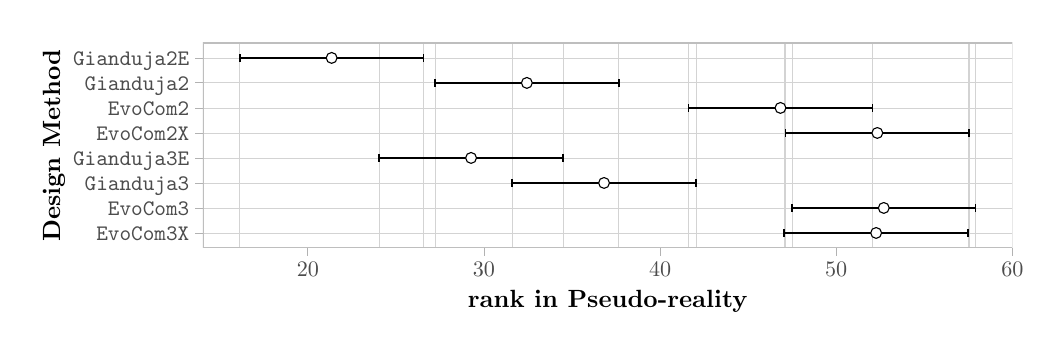
\begin{tikzpicture}[x=1pt,y=1pt]
\definecolor{fillColor}{RGB}{255,255,255}
\path[use as bounding box,fill=fillColor,fill opacity=0.00] (0,0) rectangle (361.35,108.41);
\begin{scope}
\path[clip] (  0.00,  0.00) rectangle (361.35,108.40);
\definecolor{drawColor}{RGB}{255,255,255}
\definecolor{fillColor}{RGB}{255,255,255}

\path[draw=drawColor,line width= 0.6pt,line join=round,line cap=round,fill=fillColor] (  0.00,  0.00) rectangle (361.35,108.40);
\end{scope}
\begin{scope}
\path[clip] ( 63.34, 28.81) rectangle (355.85,102.90);
\definecolor{fillColor}{RGB}{255,255,255}

\path[fill=fillColor] ( 63.34, 28.81) rectangle (355.85,102.90);
\definecolor{drawColor}{RGB}{211,211,211}

\path[draw=drawColor,line width= 0.3pt,line join=round] ( 63.34, 79.41) --
	(355.85, 79.41);

\path[draw=drawColor,line width= 0.3pt,line join=round] ( 63.34, 43.27) --
	(355.85, 43.27);

\path[draw=drawColor,line width= 0.3pt,line join=round] ( 63.34, 88.45) --
	(355.85, 88.45);

\path[draw=drawColor,line width= 0.3pt,line join=round] ( 63.34, 97.48) --
	(355.85, 97.48);

\path[draw=drawColor,line width= 0.3pt,line join=round] ( 63.34, 52.30) --
	(355.85, 52.30);

\path[draw=drawColor,line width= 0.3pt,line join=round] ( 63.34, 61.34) --
	(355.85, 61.34);

\path[draw=drawColor,line width= 0.3pt,line join=round] ( 63.34, 34.23) --
	(355.85, 34.23);

\path[draw=drawColor,line width= 0.3pt,line join=round] ( 63.34, 70.37) --
	(355.85, 70.37);

\path[draw=drawColor,line width= 0.2pt,line join=round] (305.22, 28.81) -- (305.22,102.90);

\path[draw=drawColor,line width= 0.2pt,line join=round] (340.22, 28.81) -- (340.22,102.90);

\path[draw=drawColor,line width= 0.2pt,line join=round] (213.58, 28.81) -- (213.58,102.90);

\path[draw=drawColor,line width= 0.2pt,line join=round] (143.05, 28.81) -- (143.05,102.90);

\path[draw=drawColor,line width= 0.2pt,line join=round] (342.55, 28.81) -- (342.55,102.90);

\path[draw=drawColor,line width= 0.2pt,line join=round] (339.80, 28.81) -- (339.80,102.90);

\path[draw=drawColor,line width= 0.2pt,line join=round] (241.47, 28.81) -- (241.47,102.90);

\path[draw=drawColor,line width= 0.2pt,line join=round] (193.43, 28.81) -- (193.43,102.90);

\path[draw=drawColor,line width= 0.2pt,line join=round] (238.81, 28.81) -- (238.81,102.90);

\path[draw=drawColor,line width= 0.2pt,line join=round] (273.82, 28.81) -- (273.82,102.90);

\path[draw=drawColor,line width= 0.2pt,line join=round] (147.17, 28.81) -- (147.17,102.90);

\path[draw=drawColor,line width= 0.2pt,line join=round] ( 76.64, 28.81) -- ( 76.64,102.90);

\path[draw=drawColor,line width= 0.2pt,line join=round] (276.15, 28.81) -- (276.15,102.90);

\path[draw=drawColor,line width= 0.2pt,line join=round] (273.39, 28.81) -- (273.39,102.90);

\path[draw=drawColor,line width= 0.2pt,line join=round] (175.07, 28.81) -- (175.07,102.90);

\path[draw=drawColor,line width= 0.2pt,line join=round] (127.02, 28.81) -- (127.02,102.90);
\definecolor{drawColor}{RGB}{0,0,0}

\path[draw=drawColor,line width= 0.6pt,line join=round] (305.22, 78.06) --
	(305.22, 80.77);

\path[draw=drawColor,line width= 0.6pt,line join=round] (305.22, 79.41) --
	(238.81, 79.41);

\path[draw=drawColor,line width= 0.6pt,line join=round] (238.81, 78.06) --
	(238.81, 80.77);

\path[draw=drawColor,line width= 0.6pt,line join=round] (340.22, 69.02) --
	(340.22, 71.73);

\path[draw=drawColor,line width= 0.6pt,line join=round] (340.22, 70.37) --
	(273.82, 70.37);

\path[draw=drawColor,line width= 0.6pt,line join=round] (273.82, 69.02) --
	(273.82, 71.73);

\path[draw=drawColor,line width= 0.6pt,line join=round] (213.58, 87.09) --
	(213.58, 89.80);

\path[draw=drawColor,line width= 0.6pt,line join=round] (213.58, 88.45) --
	(147.17, 88.45);

\path[draw=drawColor,line width= 0.6pt,line join=round] (147.17, 87.09) --
	(147.17, 89.80);

\path[draw=drawColor,line width= 0.6pt,line join=round] (143.05, 96.13) --
	(143.05, 98.84);

\path[draw=drawColor,line width= 0.6pt,line join=round] (143.05, 97.48) --
	( 76.64, 97.48);

\path[draw=drawColor,line width= 0.6pt,line join=round] ( 76.64, 96.13) --
	( 76.64, 98.84);

\path[draw=drawColor,line width= 0.6pt,line join=round] (342.55, 41.91) --
	(342.55, 44.62);

\path[draw=drawColor,line width= 0.6pt,line join=round] (342.55, 43.27) --
	(276.15, 43.27);

\path[draw=drawColor,line width= 0.6pt,line join=round] (276.15, 41.91) --
	(276.15, 44.62);

\path[draw=drawColor,line width= 0.6pt,line join=round] (339.80, 32.87) --
	(339.80, 35.59);

\path[draw=drawColor,line width= 0.6pt,line join=round] (339.80, 34.23) --
	(273.39, 34.23);

\path[draw=drawColor,line width= 0.6pt,line join=round] (273.39, 32.87) --
	(273.39, 35.59);

\path[draw=drawColor,line width= 0.6pt,line join=round] (241.47, 50.95) --
	(241.47, 53.66);

\path[draw=drawColor,line width= 0.6pt,line join=round] (241.47, 52.30) --
	(175.07, 52.30);

\path[draw=drawColor,line width= 0.6pt,line join=round] (175.07, 50.95) --
	(175.07, 53.66);

\path[draw=drawColor,line width= 0.6pt,line join=round] (193.43, 59.98) --
	(193.43, 62.69);

\path[draw=drawColor,line width= 0.6pt,line join=round] (193.43, 61.34) --
	(127.02, 61.34);

\path[draw=drawColor,line width= 0.6pt,line join=round] (127.02, 59.98) --
	(127.02, 62.69);

\path[draw=drawColor,line width= 0.4pt,line join=round,line cap=round,fill=fillColor] (272.02, 79.41) circle (  1.96);

\path[draw=drawColor,line width= 0.4pt,line join=round,line cap=round,fill=fillColor] (307.02, 70.37) circle (  1.96);

\path[draw=drawColor,line width= 0.4pt,line join=round,line cap=round,fill=fillColor] (180.38, 88.45) circle (  1.96);

\path[draw=drawColor,line width= 0.4pt,line join=round,line cap=round,fill=fillColor] (109.84, 97.48) circle (  1.96);

\path[draw=drawColor,line width= 0.4pt,line join=round,line cap=round,fill=fillColor] (309.35, 43.27) circle (  1.96);

\path[draw=drawColor,line width= 0.4pt,line join=round,line cap=round,fill=fillColor] (306.59, 34.23) circle (  1.96);

\path[draw=drawColor,line width= 0.4pt,line join=round,line cap=round,fill=fillColor] (208.27, 52.30) circle (  1.96);

\path[draw=drawColor,line width= 0.4pt,line join=round,line cap=round,fill=fillColor] (160.22, 61.34) circle (  1.96);
\definecolor{drawColor}{RGB}{190,190,190}

\path[draw=drawColor,line width= 0.6pt,line join=round,line cap=round] ( 63.34, 28.81) rectangle (355.85,102.90);
\end{scope}
\begin{scope}
\path[clip] (  0.00,  0.00) rectangle (361.35,108.41);
\definecolor{drawColor}{gray}{0.30}

\node[text=drawColor,anchor=base east,inner sep=0pt, outer sep=0pt, scale=  0.80] at ( 58.39, 76.66) {\texttt{EvoCom2}};

\node[text=drawColor,anchor=base east,inner sep=0pt, outer sep=0pt, scale=  0.80] at ( 58.39, 40.51) {\texttt{EvoCom3}};

\node[text=drawColor,anchor=base east,inner sep=0pt, outer sep=0pt, scale=  0.80] at ( 58.39, 85.69) {\texttt{Gianduja2}};

\node[text=drawColor,anchor=base east,inner sep=0pt, outer sep=0pt, scale=  0.80] at ( 58.39, 94.73) {\texttt{Gianduja2E}};

\node[text=drawColor,anchor=base east,inner sep=0pt, outer sep=0pt, scale=  0.80] at ( 58.39, 49.55) {\texttt{Gianduja3}};

\node[text=drawColor,anchor=base east,inner sep=0pt, outer sep=0pt, scale=  0.80] at ( 58.39, 58.58) {\texttt{Gianduja3E}};

\node[text=drawColor,anchor=base east,inner sep=0pt, outer sep=0pt, scale=  0.80] at ( 58.39, 31.48) {\texttt{EvoCom3X}};

\node[text=drawColor,anchor=base east,inner sep=0pt, outer sep=0pt, scale=  0.80] at ( 58.39, 67.62) {\texttt{EvoCom2X}};
\end{scope}
\begin{scope}
\path[clip] (  0.00,  0.00) rectangle (361.35,108.41);
\definecolor{drawColor}{gray}{0.70}

\path[draw=drawColor,line width= 0.3pt,line join=round] ( 60.59, 79.41) --
	( 63.34, 79.41);

\path[draw=drawColor,line width= 0.3pt,line join=round] ( 60.59, 43.27) --
	( 63.34, 43.27);

\path[draw=drawColor,line width= 0.3pt,line join=round] ( 60.59, 88.45) --
	( 63.34, 88.45);

\path[draw=drawColor,line width= 0.3pt,line join=round] ( 60.59, 97.48) --
	( 63.34, 97.48);

\path[draw=drawColor,line width= 0.3pt,line join=round] ( 60.59, 52.30) --
	( 63.34, 52.30);

\path[draw=drawColor,line width= 0.3pt,line join=round] ( 60.59, 61.34) --
	( 63.34, 61.34);

\path[draw=drawColor,line width= 0.3pt,line join=round] ( 60.59, 34.23) --
	( 63.34, 34.23);

\path[draw=drawColor,line width= 0.3pt,line join=round] ( 60.59, 70.37) --
	( 63.34, 70.37);
\end{scope}
\begin{scope}
\path[clip] (  0.00,  0.00) rectangle (361.35,108.41);
\definecolor{drawColor}{gray}{0.70}

\path[draw=drawColor,line width= 0.3pt,line join=round] (101.25, 26.06) --
	(101.25, 28.81);

\path[draw=drawColor,line width= 0.3pt,line join=round] (164.89, 26.06) --
	(164.89, 28.81);

\path[draw=drawColor,line width= 0.3pt,line join=round] (228.53, 26.06) --
	(228.53, 28.81);

\path[draw=drawColor,line width= 0.3pt,line join=round] (292.17, 26.06) --
	(292.17, 28.81);

\path[draw=drawColor,line width= 0.3pt,line join=round] (355.81, 26.06) --
	(355.81, 28.81);
\end{scope}
\begin{scope}
\path[clip] (  0.00,  0.00) rectangle (361.35,108.41);
\definecolor{drawColor}{gray}{0.30}

\node[text=drawColor,anchor=base,inner sep=0pt, outer sep=0pt, scale=  0.80] at (101.25, 18.35) {20};

\node[text=drawColor,anchor=base,inner sep=0pt, outer sep=0pt, scale=  0.80] at (164.89, 18.35) {30};

\node[text=drawColor,anchor=base,inner sep=0pt, outer sep=0pt, scale=  0.80] at (228.53, 18.35) {40};

\node[text=drawColor,anchor=base,inner sep=0pt, outer sep=0pt, scale=  0.80] at (292.17, 18.35) {50};

\node[text=drawColor,anchor=base,inner sep=0pt, outer sep=0pt, scale=  0.80] at (355.81, 18.35) {60};
\end{scope}
\begin{scope}
\path[clip] (  0.00,  0.00) rectangle (361.35,108.41);
\definecolor{drawColor}{RGB}{0,0,0}

\node[text=drawColor,anchor=base,inner sep=0pt, outer sep=0pt, scale=  0.90] at (209.60,  7.44) {\bfseries rank in Pseudo-reality};
\end{scope}
\begin{scope}
\path[clip] (  0.00,  0.00) rectangle (361.35,108.41);
\definecolor{drawColor}{RGB}{0,0,0}

\node[text=drawColor,rotate= 90.00,anchor=base,inner sep=0pt, outer sep=0pt, scale=  0.90] at ( 11.71, 65.86) {\bfseries Design Method};
\end{scope}
\end{tikzpicture}
